% This must be in the first 5 lines to tell arXiv to use pdfLaTeX, which is strongly recommended.
\pdfoutput=1
% In particular, the hyperref package requires pdfLaTeX in order to break URLs across lines.

\documentclass[11pt]{article}

% Remove the "review" option to generate the final version.
\usepackage[]{acl}

% Standard package includes
\usepackage{times}
\usepackage{latexsym}
\usepackage{graphicx}


% For proper rendering and hyphenation of words containing Latin characters (including in bib files)
\usepackage[T1]{fontenc}
% For Vietnamese characters
% \usepackage[T5]{fontenc}
% See https://www.latex-project.org/help/documentation/encguide.pdf for other character sets

% This assumes your files are encoded as UTF8
\usepackage[utf8]{inputenc}

% This is not strictly necessary, and may be commented out,
% but it will improve the layout of the manuscript,
% and will typically save some space.
\usepackage{microtype}

\usepackage{listings}
\usepackage{xcolor}

\lstdefinelanguage{nGQL}{
  morekeywords={GO, FROM, OVER, REVERSELY, WHERE, CONTAINS, YIELD, AS},
  sensitive=true,
  morecomment=[l]{--},
  morestring=[b]",
}

\lstset{
  language=nGQL,
  backgroundcolor=\color{black!5},
  basicstyle=\ttfamily\small,
  keywordstyle=\color{blue}\bfseries,
  commentstyle=\color{gray}\itshape,
  stringstyle=\color{olive},
  showstringspaces=false,
  columns=flexible,
  keepspaces=true,
  frame=single,
  breaklines=true,
}

% If the title and author information does not fit in the area allocated, uncomment the following
%
%\setlength\titlebox{<dim>}
%
% and set <dim> to something 5cm or larger.

\title{A Comprehensive Study on Multimodal In-Context Learning for BI Charts and Reports}

% Author information can be set in various styles:
% For several authors from the same institution:
% \author{Author 1 \and ... \and Author n \\
%         Address line \\ ... \\ Address line}
% if the names do not fit well on one line use
%         Author 1 \\ {\bf Author 2} \\ ... \\ {\bf Author n} \\
% For authors from different institutions:
% \author{Author 1 \\ Address line \\  ... \\ Address line
%         \And  ... \And
%         Author n \\ Address line \\ ... \\ Address line}
% To start a seperate ``row'' of authors use \AND, as in
% \author{Author 1 \\ Address line \\  ... \\ Address line
%         \AND
%         Author 2 \\ Address line \\ ... \\ Address line \And
%         Author 3 \\ Address line \\ ... \\ Address line}

\author{
\begin{tabular}{ccc}
\textbf{Akhil Srivatsava} & \textbf{Bimal Dev} & \textbf{Prashant Agarwal} \\
\texttt{sriakhil25@gmail.com} & \texttt{bimal.d3v@gmail.com} & \texttt{prashant.agarwal92@gmail.com} \\
\end{tabular}
}


\begin{document}

\maketitle

\section*{General problem/task definition}
Business Intelligence (BI) reports today often blend charts, tables, and explanatory text, making interpretation a cognitively demanding task. As this data becomes increasingly multimodal, there’s a growing need for models that can reason across both visual and textual formats. Multimodal Large Language Models (MLLMs) offer a strong foundation for this, combining vision and language within a shared reasoning framework. At a high level, these systems function much like human cognition: the LLM operates as the decision engine, while modality encoders work like sensors that translate visuals—such as charts and layout—into textual embeddings via projectors that align otherwise disjoint embedding spaces.

In this review, we examine nine recent contributions in chart-focused MLLMs, such as UniChart, ChartAssistant, and ChartInstruct. These models aim to overcome well-known limitations in general-purpose systems like GPT-4V and CLIP, which often struggle with structured visuals due to weak visual-semantic grounding and poor numerical reasoning. We classify MLLM capabilities along three core axes: (1) general multimodal reasoning (object recognition, OCR, spatial understanding), (2) trust and reliability (robustness, hallucination resistance, safety), and (3) task-specific effectiveness (e.g., chart question answering, summarization, chart-to-table conversion). Our evaluation of top-tier MLLMs—GPT-4o, Claude 3 Opus, and Gemini 1.5 Pro—across benchmarks like VLAT and MMBench shows wide performance swings and persistent issues like confusion between color and semantics, spatial misinterpretation, and difficulty handling chart scales. While these models generally perform well on trends and high-level insights, they often miss fine-grained tasks like outlier detection or precise value extraction.

Motivated by these findings, we outline a new system architecture tailored for BI applications: a Graph-based Retrieval-Augmented Generation (Graph RAG) framework optimized for multimodal in-context learning. The design integrates LayoutLMv3 to capture layout-aware document structure, and combines NebulaDB, vector search, and precomputed similarity graphs for hybrid retrieval. This setup avoids typical pitfalls of ANN-based methods (e.g., HNSW and Navigable Small World Graphs), instead supporting deterministic metadata filtering and explainable graph traversal to boost accuracy, speed, and transparency—critical requirements in enterprise-scale BI settings.

Our review highlights a gap in current systems: no existing model fully tackles the combined challenges of layout modeling, multimodal alignment, and in-context reasoning in BI workflows. We advocate for a cohesive architecture that merges structural modeling from ChartAssistant, UniChart’s lightweight task-driven tuning, and the instructional flexibility seen in ChartInstruct. Looking ahead, the path forward includes exploring layout-aware chain-of-thought prompting, visually grounded CoT reasoning, and establishing evaluation standards to benchmark MLLMs in real-world analytics environments.

\section*{Concise summaries of the articles}

\paragraph{UniChart:} UniChart is a pretrained model specifically designed for chart comprehension and reasoning. It introduces a novel architecture with a Swin Transformer-based chart encoder and a BART text decoder. Trained on over 611K diverse charts, it combines low-level tasks (like visual element extraction) with high-level reasoning (e.g., question answering and summarization). It achieves state-of-the-art performance across multiple chart-related benchmarks (ChartQA, Chart-to-Text, OpenCQA, Chart-to-Table) and improves efficiency through linear-scaling attention. Despite its strengths, UniChart struggles with compositional reasoning and generalization to unseen chart formats.

\paragraph{ChartAssistant:} ChartAssistant is a multitask vision-language model tailored for chart understanding, trained on ChartSFT, a large-scale dataset with over 24 million samples across diverse tasks (chart-to-table, numerical QA, summarization). It employs a two-stage training process: chart-to-table pretraining and multitask instruction tuning. ChartAssistant is implemented in two variants: ChartAst-D (efficient) and ChartAst-S (generalizable). The model outperforms UniChart and even GPT-4V in numerical and referring QA, with strong generalization to specialized chart types. Ablation studies highlight the importance of alignment pretraining, Chain-of-Thought (CoT) reasoning, and referring QA in driving model performance.

\paragraph{ChartInstruct:} ChartInstruct introduces a large-scale instruction-tuned dataset of 191K examples from 71K charts for improving chart reasoning and generation. The dataset includes tasks such as summarization, fact-checking, CoT reasoning, and Python code generation. Two modeling approaches are proposed: an end-to-end system using UniChart as the visual encoder, and a pipeline model that first extracts structured chart data. Evaluations demonstrate improved performance across a wide range of chart-related tasks and highlight the effectiveness of using diverse, real-world instructions. ChartInstruct focuses more on instructional breadth than architectural novelty.

\paragraph{GPT-4V and MLLMs on Visualization Literacy:} Several studies have empirically evaluated multimodal LLMs like GPT-4V, Claude 3 Opus, and Gemini 1.5 Pro on visualization-centric tasks. While these models exhibit strength in identifying high-level trends, clusters, and comparisons, they consistently underperform humans in value retrieval, pie chart interpretation, and color-semantic disambiguation. For example, GPT-4V placed in the 16th percentile on the VLAT benchmark. These results underscore the importance of visual grounding and structured reasoning for accurate chart interpretation.

\paragraph{MM-GEM and Layout-LMV3:}

Two components involved in RAG retrieval 1)Vector Embeddings 2)Vector DBs. We are working on limitations of both components.

1. Problems with Clip Embeddings - We are choosing LayoutLMv3 and initially considered MMGEM as well but we found limitations
2. Limitations of Vector DB Search - papers around ANN and HNSW

Choosing Embeddings for Multi Modal RAG

We initially considered MM-GEM (MultiModal Generative Embedding Model) and went through its paper but found it to be not good for our use case:

MM-GEM (MultiModal Generative Embedding Model) offers a unified architecture that jointly supports both retrieval and generation. It aligns image regions and textual spans within a shared embedding space, delivering strong performance on image-text retrieval tasks, with Recall@1 scores exceeding CLIP on datasets like COCO and Flickr. Built using ViT-Large and TinyLlama, MM-GEM's design is well-suited for end-to-end production RAG pipelines. However, it lacks layout-awareness—a crucial requirement for enterprise document understanding—and has no publicly available pretrained checkpoints, making integration and reproducibility challenging.


Challenges :

- No pretrained model publicly available (not on HuggingFace, Ollama, etc.)
- No layout awareness — it doesn’t handle document structure like tables, charts, or token-to-region mapping.


We finally decided to choose LayoutLMv3 for our MultiModal RAG QA 

LayoutLMv3, by contrast, is a layout-aware transformer model that integrates text, image, and spatial layout signals using a single Vision Transformer (ViT) backbone. It enables fine-grained token-to-region mapping, making it ideal for structured documents like tables, forms, and business charts. By jointly modeling OCR text and document visuals, LayoutLMv3 achieves state-of-the-art results on tasks like document question answering and information extraction. Given its layout sensitivity and availability on platforms like HuggingFace, LayoutLMv3 is a more practical and accurate choice for multimodal RAG applications in BI/analytics settings.

\paragraph{The survey paper on Vector Databases (VDBs)}
highlights fundamental limitations in current Vector Databases (VDBs) that rely on Approximate Nearest Neighbor (ANN) methods like HNSW for similarity search. While ANN algorithms offer fast retrieval, they struggle to scale efficiently as the number of vectors grows into the billions. Moreover, they lack explainability, making it difficult to trace why a particular result was retrieved—an issue critical for enterprise applications. ANN-based systems also fall short in supporting structured metadata filtering, which limits context-aware search. These constraints—scalability, transparency, and semantic filtering—make traditional ANN pipelines brittle for high-stakes use cases like BI/Analytics. This lays the foundation for our Graph RAG approach, which combines metadata filtering, graph traversal, and precomputed similarity links to enable deterministic, interpretable, and semantically scoped retrieval, overcoming the inherent drawbacks of ANN and HNSW-based search.


\section*{Compare and contrast} 

\paragraph{Architectural Strategies:}
All three core models—UniChart, ChartAssistant, and ChartInstruct—attempt to address the same core challenge: enabling robust chart comprehension via multimodal large language models (MLLMs). However, they differ in how they architect for this. UniChart uses a Donut-style encoder-decoder model with chart-specific pretraining objectives. ChartAssistant leverages a two-stage approach: chart-to-table translation followed by multitask instruction tuning. It is implemented in two variants: a compact version (ChartAst-D) and a large generalizable model (ChartAst-S) based on SPHINX. ChartInstruct, by contrast, does not introduce a novel model architecture but instead focuses on enriching model performance through a diverse, instruction-tuned dataset for chart-related tasks.

\paragraph{Data and Pretraining Scale:}
UniChart is trained on 611K charts sourced from web data, SVG extractions, and synthetic generation pipelines. ChartAssistant, built on the ChartSFT benchmark, uses over 24 million samples spanning a range of tasks, including numerical QA and chart summarization. ChartInstruct includes 191K instructions generated from 71K charts and uniquely emphasizes real-world and diverse instructional prompts, including novel tasks like code generation and fact-checking. In terms of scale, ChartAssistant leads in training volume, while ChartInstruct offers the most diverse instruction set.

\paragraph{Task Coverage and Flexibility:}
All three models support key downstream tasks: chart summarization, chart QA (both visual and numerical), and chart-to-table translation. However, ChartAssistant extends its capabilities to complex tasks like referring QA and CoT (Chain-of-Thought) reasoning, where UniChart and GPT-4V show limited ability. ChartInstruct introduces novel tasks (e.g., chart-based code generation) not addressed in the others. This positions ChartInstruct as the most task-diverse, ChartAssistant as the most reasoning-capable, and UniChart as a lightweight, efficient baseline.

\paragraph{Evaluation Methodology:}
UniChart and ChartAssistant are evaluated on established benchmarks such as ChartQA, OpenCQA, and Chart-to-Text, with performance reported using both automated metrics (BLEU, Relaxed Accuracy) and human studies. ChartAssistant outperforms prior models—including GPT-4V and Bard—on multiple chart understanding tasks, particularly in numerical and referring QA. ChartInstruct complements this by demonstrating strong human-aligned reasoning through diverse instruction evaluation. Additionally, GPT-4V’s performance on VLAT reveals a clear discrepancy between high-level reasoning (strong) and low-level visual interpretation (weak), exposing gaps in current general-purpose MLLMs.

\paragraph{Generalization and Robustness:}
UniChart struggles with compositional reasoning and unfamiliar chart types. ChartAssistant shows strong generalization across both base and specialized chart formats due to its scale and multitask training. ChartInstruct enhances real-world robustness by incorporating diverse prompts from real chart scenarios. Evaluation studies of GPT-4V and other MLLMs on visualization literacy tests highlight instability across question types and sensitivity to prompt wording, emphasizing the need for stronger visual-semantic alignment and layout awareness.

\paragraph{Instruction Tuning vs. Model Architecture:}
ChartAssistant and UniChart rely heavily on architectural innovations—visual encoders, pretraining objectives, and token-level reasoning. ChartInstruct, on the other hand, exemplifies how dataset quality and instruction diversity alone can significantly improve multimodal reasoning. This decouples performance gains from model size or architecture, suggesting that instruction tuning—if sufficiently diverse—can rival task-specific pretraining in many scenarios.

\paragraph{LayoutLMv3 vs MM-GEM}
In comparing LayoutLMv3 + LLM with MM-GEM for our retrieval pipeline, several practical advantages favor the former. LayoutLMv3 offers excellent document layout-aware extraction, crucial for handling forms, tables, and structured business reports—something MM-GEM lacks due to its absence of token-level layout awareness. For PDFs and charts, LayoutLMv3 integrates well with segmentation models like YOLO or Detectron2 and OCR models like BLIP, whereas MM-GEM would require end-to-end unified training for the same. In terms of fine-grained OCR text mapping, LayoutLMv3 provides precise bounding box alignment, while MM-GEM focuses more broadly on visual regions without structured mapping. Another key differentiator is modularity—LayoutLMv3 allows flexible LLM pairing and easy experimentation, unlike MM-GEM's tightly coupled architecture. Additionally, LayoutLMv3 is readily available with pretrained weights on HuggingFace, enabling immediate integration, while MM-GEM lacks public checkpoints. Lastly, for deployment and scalability, LayoutLMv3 supports modular, CPU-friendly setups, whereas MM-GEM requires a more heavyweight, full-stack environment, making it less suitable for production BI workflows.

\paragraph{VectorDB vs GraphRAG}
Compared to standard vector databases like HNSW, the hybrid approach combining NebulaDB with Vector DB offers several advantages critical for enterprise-scale retrieval. While HNSW provides fast ANN search, it operates over the entire vector set, often retrieving semantically irrelevant results. In contrast, the hybrid setup uses metadata-based pre-filtering, enabling faster, context-aware and more accurate retrieval. It also enhances explainability by leveraging graph schemas and metadata traceability, which HNSW lacks. Furthermore, the hybrid design supports robust structured filtering through nGQL traversal and scales more efficiently by reducing the candidate pool before similarity search—addressing a key limitation in HNSW’s performance at large scale.

Most current RAG implementations rely on approximate nearest neighbor (ANN) search using vector databases like FAISS or HNSW, which—while fast—struggle with semantic relevance, scalability, and explainability. In contrast, our proposed architecture leverages a hybrid approach combining NebulaDB for graph-based filtering with a standard vector database and precomputed similarity scores. This design enables structured, context-aware retrieval through metadata constraints extracted by an LLM (e.g., filtering for "Geography: US"), which significantly narrows the candidate space before vector similarity is applied. As a result, our system improves retrieval accuracy, explainability (via graph traceability), and performance on large-scale, structured BI data—addressing key limitations identified in existing ANN-based methods.

\begin{lstlisting}[caption={Graph-Based Filtering with nGQL (O(1))}]
GO FROM (
  GO FROM ["US"] OVER BELONGS_TO REVERSELY
    WHERE ["Geography"] CONTAINS $^.Metadata.type
) OVER BELONGS_TO YIELD dst AS chunkID;
\end{lstlisting}

A key innovation in our Graph RAG architecture is the narrowing of the search space from all document chunks (N) to a highly relevant subset (M $\ll$ N) through graph-based filtering. By applying metadata constraints (e.g., domain-specific filters like Geography = US), we perform vector similarity search only on contextually relevant chunks. This two-stage process drastically reduces retrieval noise, improves semantic alignment, and leads to lower latency and higher accuracy. Furthermore, it enhances explainability by ensuring results are grounded in both semantic similarity and structured metadata relationships—offering a significant edge over traditional ANN-only approaches.


\paragraph{Summary.}
While all models aim to improve chart understanding, they diverge in approach:
\begin{itemize}
    \item \textbf{UniChart} prioritizes architectural efficiency and task-specific pretraining.
    \item \textbf{ChartAssistant} demonstrates the strongest performance across tasks through extensive instruction tuning and robust model scaling.
    \item \textbf{ChartInstruct} excels in data diversity and instructional generalization, offering the broadest task coverage with minimal architectural changes.
    \item \textbf{GPT-4V and other MLLMs} show promise in trend and pattern recognition but fall short in fine-grained perception and grounded reasoning.
\end{itemize}

The landscape suggests future models should hybridize: leveraging ChartAssistant’s structured alignment, UniChart’s lightweight inference efficiency, and ChartInstruct’s diverse instructional tuning—possibly enhanced with layout-aware encoders like LayoutLMv3 to improve spatial understanding.


\section*{Future work}

\paragraph*{Graph RAG Retrieval \& Ranking:}

To address retrieval quality and scalability in enterprise BI systems, we propose a Graph-based Retrieval-Augmented Generation (Graph RAG) framework.

\paragraph{A) Hybrid Search Process.}
\begin{itemize}
    \item \textbf{Metadata Filtering (O(1))} – Fast, deterministic filtering using NebulaDB's nGQL metadata queries.
    \item \textbf{Embedding Similarity Search (O(K))} – Performed only on filtered results using KNN or ANN.
    \item \textbf{Multi-hop Expansion} – Graph traversal retrieves SIMILAR\_TO and NEXT-connected chunks to improve context richness.
\end{itemize}

\paragraph{B) nGQL Execution Logic.}
\begin{itemize}
    \item With metadata: first filter (O(1)), then vector similarity search.
    \item Without metadata: vector similarity search is performed directly.
    \item Optional multi-hop expansion enhances retrieval quality.
\end{itemize}

\begin{figure}[h]
  \centering
  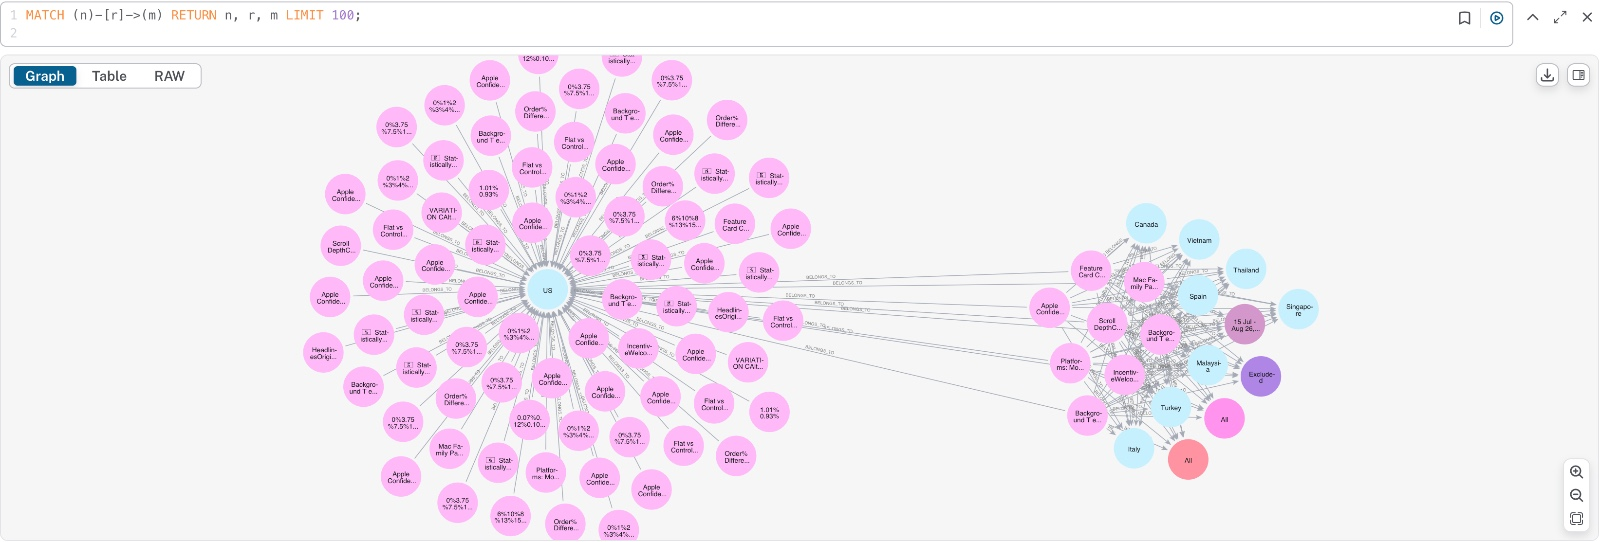
\includegraphics[width=\linewidth]{graph_rag_img.jpeg}
  \caption{Graph RAG retrieval and expansion process with layout-aware context}
  \label{fig:graph_rag}
\end{figure}

\subsection*{LayoutLMv3 for BI, PDFs, and Structured Visual QA}

\textbf{Why LayoutLMv3?} Traditional embeddings like CLIP lack spatial and structural sensitivity critical for structured BI reports. LayoutLMv3 integrates text, layout, and vision at the token level using a unified transformer with a Vision Transformer (ViT) backbone.

\textbf{Key Features:}
\begin{itemize}
    \item Token-to-bounding box mapping enables spatial grounding.
    \item Fine-grained embeddings make it ideal for forms, tables, and PDFs.
    \item Compatible with OCR-based QA systems (e.g., BLIP, Donut).
\end{itemize}

\textbf{Future Directions:}
\begin{itemize}
    \item Efficient chunking of long BI documents using layout segmentation.
    \item Multi-hop graph traversal with CoT-style visual reasoning.
    \item Development of benchmark tasks combining layout QA, chart reasoning, and in-context retrieval validation.
    \item Visualization of retrieval paths and chunk-level confidence scoring for explainability.
\end{itemize}



% Entries for the entire Anthology, followed by custom entries
\nocite{masry2023unichart, zhang2024chartassistant, lin2024chartinstruct, li2024visualizationliteracy, bendeck2024gpt4vis, huang2024survey, huang2023layoutlmv3, zhang2024mmgem, liu2023vectordbsurvey}
\bibliographystyle{acl_natbib}
\bibliography{anthology,custom}

\end{document}
